\chapter{Service 1}
\section{classe User implémente en java  }

\begin{lstlisting}[language=java]
 import javax.persistence.Entity;
 import javax.persistence.GeneratedValue;
 import javax.persistence.Id;
 import java.io.Serializable;
 
 @Entity
 public class User implements Serializable {
 @Id
 @GeneratedValue
 private int id;
 private String name;
 public user(){
 }
 public user(String name) {
 this.name = name;
 }
 public int getId() {
 return id;
 }
 public void setId(int id) {
 this.id = id;
 }
 public String getName() {
 return name;
 }
 public void setName(String name) {
 this.name = name;
 }
 }
\end{lstlisting}

\section{créer l'interface UserRepository}


\begin{lstlisting}[language=java]
import org.springframework.data.jpa.repository.
JpaRepository;

public interface userRepository extends JpaRepository<user , Integer>{ 
}
\end{lstlisting}


\section{classe DummyDataCLR en java }
\begin{lstlisting}[language=java]
 

import org.springframework.beans.factory.annotation.Autowired;
import org.springframework.boot.CommandLineRunner;
import org.springframework.stereotype.Component;

import java.util.stream.Stream;

@Component
class DummyDataCLR implements CommandLineRunner {

@Override
public void run(String... strings) throws Exception {
Stream.of("Pencil", "Book", "Eraser").forEach(s->userRepository.save(new user(s)));
userRepository.findAll().forEach(s->System.out.println(s.getName()));
}

@Autowired
private userRepository userRepository;

}
\end{lstlisting}

\chapter{ConfigService}
 
\section{classe ConfigServiceApplication en java }
   \begin{lstlisting}[language=java]
   import org.springframework.boot.SpringApplication;
   import org.springframework.boot.autoconfigure.
   SpringBootApplication;
   import org.springframework.cloud.config.server.
   EnableConfigServer;
   
   @EnableConfigServer
   @SpringBootApplication
   public class ConfigServiceApplication {
   
   public static void main(String[] args) {
   
   SpringApplication.run(ConfigServiceApplicatin.class, args);
   }
   }
   \end{lstlisting} 
   
 \ 
  
 \section{json }
       \begin{lstlisting} 
       {
       name: "service-1",
       profiles: [
       "master"
       ],
       label: null,
       version: "6e1ea61d706133e2d8b62f40c6b784192fb58e8a",
       state: null,
       propertySources: [
       {
       name: "file:./src/main/resources/myConfig/application.properties",
       source: {
       global: "xxxxx"
       }
       }
       ]
       }
         \end{lstlisting}
        
          \section{json }
              \begin{lstlisting}
        {
        	name: "service-1",
        	profiles: [
        	"master"
        	],
        	label: null,
        	version: "6e1ea61d706133e2d8b62f40c6b784192fb58e8a",
        	state: null,
        	propertySources: [
        	{
        		name: "file:./src/main/resources/myConfig/user-service.properties",
        		source: {
        			me: "Djamel.Zerrouki@jimmi.fr"
        		}
        	},
        	{
        		name: "file:./src/main/resources/myConfig/application.properties",
        		source: {
        			global: "xxxxx"
        		}
        	}
        	]
        } 
        \end{lstlisting}
        
       \section{classe userRestService en java }
      \begin{lstlisting}
import  org.springframework.beans.factory.annotation.Value;
import org.springframework.web.bind.annotation.RequestMapping;
import org.springframework.web.bind.annotation.RestController;

@RestController
public class userRestService {

@Value("${me}")
private String me;

@RequestMapping("/messages")
public String tellMe(){
System.out.println("c'est moi qui ai repondu!");
return me;
}
}
      \end{lstlisting}  
        
        
  \chapter*{L'organigramme de la CNR}
        
\begin{figure}[H]
	\centering
	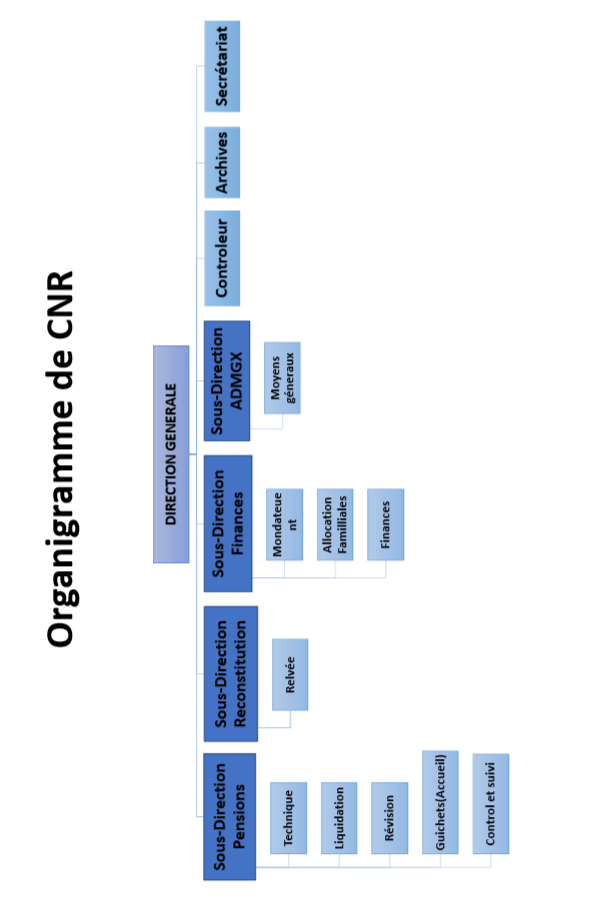
\includegraphics[width=1\linewidth,height=0.58\paperheight]{images/orgpdf}
	\caption{L'organigramme de la CNR}
	\label{fig:orgpdf}
\end{figure}
